\section{Theorie}

\subsection{Kohärenzlänge und Kohärenzzeit}
Unter der Kohärenzlänge einer Lichtquelle versteht man die Länge, um die sich die durchlaufenen Wege zweier von der selben Lichtquelle stammenden Strahlen maximal unterscheiden dürfen, sodass noch eine räumlich und zeitlich konstante Interferenz zu beobachten ist. Grund hierfür ist, dass einige Lichtquellen keine über längere Zeit exakte Sinusschwingung liefern, sondern sich mit der Zeit ein \enquote{Versatz} der Phase herausbildet. Es ist also nicht mehr möglich, für eine Länge zwischen einem Maximum und einem weiteren Punkt auf dem Wellenzug, die zwar einem Vielfachen der Wellenlänge entspricht, aber auch die Kohärenzlänge überschreitet, wiederum auf ein Maximum zu schließen. \\
Die Kohärenzzeit bezeichnet die maximale Zeitdifferenz zwischen zwei Punkten auf dem Wellenzug, deren Abstand kleiner als die Kohärenzlänge ist, und ergibt sich deshalb im Vakuum zu 

\begin{equation}
t_{K} = \frac{l_{k}}{c},
\end{equation}

wobei hier $ t_{K} $ die Kohärenzzeit, $ l_{k} $ die Kohärenzlänge und c die Lichtgeschwindigkeit bezeichnet. \\
Bei Lasern ist die Kohärenzlänge meist verhältnismäßig groß und kann mehrere Kilometer erreichen, wohingegen bei anderen Lichtquellen, die etwa auf thermischer Emission beruhen, nur sehr kleine Kohärenzlängen erreicht werden. So liegt diese bei Glühbirnen im Bereich von Mikrometern. 

\subsection{Interferenz zweier Lichtstrahlen}
Werden zwei Lichtstrahlen, die in gleicher Richtung polarisiert sind, überlagert, so ergibt sich die tatsächliche Lichteinstrahlung durch Addition der beiden elektrischen Felder an diesem Ort. 
Seien $ \vec{E}_{1} $ und $ \vec{E}_{2} $ die elektrischen Felder des einfallenden Lichts mit: 
\begin{equation}
\vec{E}_{1} = \vec{e}_{p} \cdot E_{1} \cdot e^{i(\omega_{1}t - k_{1} \cdot r + \phi_{1})}
\end{equation} und 
\begin{equation}
\vec{E}_{2} = \vec{e}_{p} \cdot E_{2} \cdot e^{i(\omega_{2}t - k_{2} \cdot r + \phi_{2})}.
\end{equation}

Dabei sind $ E_{1}, E_{2} $ die Amplituden beider Felder, $ \omega_{1}, \omega_{2} $ die Frequenzen der beiden Schwingungen, $ r_{1}, r_{2} $ die zurückgelegten Wege der beiden Lichtstrahlen, $ k_{1}, k_{2} $ die Beträge der Wellenvektoren $ \vec{k_{1}}, \vec{k_{2}} $, der in Ausbreitungsrichtung zeigen soll und $ \vec{e}_{p} $ der Einheitsvektor in Richtung der Polarisation. Weiter sind  $ \phi_{1} $ und $ \phi_{2} $ die Phasen des elektrischen Feldes bei $ r_{1}, r_{2}, t = 0 $. 
 
Als Summe über beide Felder ergibt sich zeitabhängig: 
\begin{equation}
\vec{E}_{1} + \vec{E}_{2} = \vec{e}_{p} \cdot (E_{1} \cdot e^{i(\omega_{1}t - k_{1} \cdot r_{1} + \phi_{1})} + E_{2} \cdot e^{i(\omega_{2}t - k_{2} \cdot r_{2} + \phi_{2})}).
\end{equation}

Mit $ \varphi_{1} = - k_{1} \cdot r_{1} + \phi_{1} $ und 
$ \varphi_{2} = - k_{2} \cdot r_{2} + \phi_{2} $ ergibt sich: 
\begin{equation}
\vec{E} = \vec{E}_{1} + \vec{E}_{2} = \vec{e}_{p} \cdot (E_{1} \cdot e^{i(\omega_{1}t + \varphi_{1})} + E_{2} \cdot e^{i(\omega_{2}t + \varphi_{2})}).
\end{equation}
Die Lichtintensität I ist bekanntlich proportional zum zeitlichen Mittel von $ | \vec{E}_{reell} |^{2} $ über eine Schwingung, deshalb: 

\begin{equation}
\nonumber
| \vec{E}_{reell} |^{2} = 
|(\vec{e}_{p} \cdot (E_{1} \cdot \cos(\omega_{1}t + \varphi_{1})) + E_{2} \cdot \cos(\omega_{2}t + \varphi_{2})))|^{2} = 
(E_{1} \cdot \cos(\omega_{1}t + \varphi_{1}) + E_{2} \cdot \cos(\omega_{2}t + \varphi_{2}))^{2} = 
\end{equation}
\begin{equation}
E_{1}^{2} \cdot cos^{2}(\omega_{1}t + \varphi_{1}) + 2E_{1}E_{2} \cdot \cos(\omega_{1}t + \varphi_{1}) \cdot \cos(\omega_{2}t + \varphi_{2}) + E_{2}^{2} \cdot \cos^{2}(\omega_{2}t + \varphi_{2}).
\end{equation}


Die beiden quadratischen Terme können als Feldstärkequadrate der einzelnen Strahlen identifiziert werden, es bleibt der Mischterm: 
\begin{equation}
2E_{1}E_{2} \cdot \cos(\omega_{1}t + \varphi_{1}) \cdot \cos(\omega_{2}t + \varphi_{2}) = 
E_{1}E_{2} \cdot (\cos(t(\omega_{1} + \omega_{2}) + \varphi_{1} + \varphi_{2}) + \cos(t(\omega_{1} - \omega_{2}) + \varphi_{1} - \varphi_{2})).
\end{equation}
Für $ \omega_{1} = \omega_{2} $ (und damit auch $ k_{1} = k_{2} $) kann dies weiter vereinfacht werden zu: 
\begin{equation}
E_{1}E_{2} \cdot (\cos(2\omega t + \varphi_{1} + \varphi_{2}) + \cos(\varphi_{1} - \varphi_{2})),
\end{equation} für $ \omega_{1} \neq \omega_{2} $ würde sich im längerfristigen zeitlichen Mittel über dem Mischterm 0 ergeben, da beide Summanden zeitabhängig wären. 


Mittelt man nun über $ | \vec{E}_{reell} |^{2} $, so folgt: 
\begin{equation}
\nonumber
<| \vec{E}_{reell} |^{2}> = 
\end{equation}
\begin{equation}
\nonumber
< E_{1}^{2} \cdot cos^{2}(\omega_{1}t + \varphi_{1}) + E_{2}^{2} \cdot \cos^{2}(\omega_{2}t + \varphi_{2}) + E_{1}E_{2} \cdot (\cos(2\omega t + \varphi_{1} + \varphi_{2}) + \cos(\varphi_{1} - \varphi_{2})) > = 
\end{equation}
\begin{equation}
\nonumber
\frac{E_{1}^{2}}{2} + \frac{E_{2}^{2}}{2} + E_{1}E_{2} \cdot \cos(\varphi_{1} - \varphi_{2}) = 
\end{equation}
\begin{equation}
\frac{E_{1}^{2}}{2} + \frac{E_{2}^{2}}{2} + E_{1}E_{2} \cdot \cos( k \cdot (r_{2} - r_{1}) + \phi_{1} - \phi_{2}).
\end{equation}

Bezeichnen $ I_{1}, I_{2} $ die Intensitäten der einfallenden Lichtstrahlen, so ergibt sich über $ I = \mu <|\vec{E}_{reell}|^{2}> $: 
\begin{equation}
\label{formel:intensitaet}
I = I_{1} + I_{2} + 2 \sqrt{I_{1} I_{2}} \cdot \cos( k \cdot (r_{2} - r_{1}) + \phi_{1} - \phi_{2}).
\end{equation}





\subsection{Das Michelson-Interferometer}

Das Michelson-Interferometer gehört zur Klasse der Zweistrahlinterferometer. Seine Funktionsweise beruht darauf, dass ein polarisierter Laserstrahl mit Hilfe eines halbdurchlässigen Spiegels aufgespalten wird (siehe dazu Abb. \ref{pic:skizze_versuchsaufbau}). Beide Strahlen werden gespiegelt und so wieder am halbdurchlässigen Spiegel vereinigt. Aufgrund der unterschiedlich großen zurückgelegten Wegstrecken kommt es dort zu Interferenzeffekten, die vom genauen Aufbau des Interferometers abhängen.\\
Verändert man die Länge von einem der beiden Wege, so ändert sich auch die Phasenverschiebung zwischen beiden Lichtstrahlen und nach (\ref{formel:intensitaet}) auch die Intensität der interferierenden Strahlen und bildet eine sinusförmige Kurve. Durch Beobachtung der Verschiebung der Interferenzen kann also auf die Geschwindigkeit geschlossen werden, mit der sich die Länge des einen Weges ändert: 
Hat sich das Interferenzmuster genau um $ 2 \pi $ verschoben, so hat sich nach (\ref{formel:intensitaet}) $ k \cdot \Delta r $ um $ 2 \pi $ vergrößert oder verkleinert.
Ein $ \Delta N $ von 1 entspricht deswegen genau einer Längenänderung um $ \frac{\lambda}{2} $, also:


\begin{equation}
\Delta l = \frac{\lambda}{2} \cdot \Delta N. 
\end{equation}


wobei $ \lambda $ die Wellenlänge des verwendeten Lasers ist und N die Anzahl der während der Längenänderung \enquote{vorbeigelaufenen} Ringe ist. 



Weiterhin kann das vom Laser emittierte Strahlenbündel durch Einbringen von einer oder mehrerer Linsen zu einem divergenten Strahl oder einem breiteren, parallelen Strahlenbündel gewandelt werden. Oftmals geschieht dies mit Hilfe eines \enquote{Teleskops}, bei dem das Strahlenbündel eine Kombination aus konkaver und konvexer Linse durchläuft und danach parallel austritt. Im Falle eines zu Beginn ebenfalls parallelen Strahlenbündels, wie es vom Laser in guter Näherung emittiert wird, müssen dazu offenbar die beiden Brennpunkte aufeinander fallen.  \\

Die beobachtbaren Interferenzeffekte hängen maßgeblich von der genauen Ausrichtung der optischen Elemente im Strahlengang ab: 
Sind etwa die reflektierenden Spiegel nicht exakt senkrecht zum einfallenden Strahl ausgerichtet oder der halbdurchlässige Spiegel nicht in einem Winkel von exakt $ 45 ^\circ$  zum einfallenden Strahl justiert, so führt diese Verkippung der Spiegel zu deutlich sichtbaren Interferenzstreifen, da die Wellenfronten der beiden interferierenden Strahlen dann nicht parallel auf den Schirm treffen. (Abb. \ref{verkippung}: Die Differenz zwischen den beiden gestrichelten Strecken entspricht dem Phasenversatz zwischen den beiden Wellen an dem entsprechenden Punkt auf dem Schirm. Der Versatz ändert sich in der Horizontalen.) Treffen sich weiter die beiden Strahlbündel bei Vereinigung auf dem halbdurchlässigen Spiegel nicht mittig am gleichen Punkt, so beobachtet man sehr deutlich Interferenzringe, da sich die Laufzeiten bei Verschieben des betrachteten Punkts unterschiedlich ändern. 

\begin{figure}
\centering
        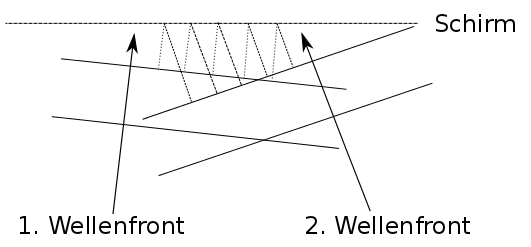
\includegraphics[width=.9\textwidth]{images/verkippung.png}
\caption{Darstellung der Interferenz zwischen zwei verkippten Wellenfronten}
\label{verkippung}
\end{figure}


\subsection{Thermische Längenänderung}
Wird ein Material erhitzt, so dehnt es sich in den meisten Fällen aus. Dies kann im Standard-Atom-Modell für einen Feststoff veranschaulicht werden: Wird dem Stoff thermische Energie zugeführt, bedeutet dies effektiv eine Zunahme der kinetischen Energie der Atomrümpfe. Dadurch nimmt die Amplitude von deren Schwingung um die Ruhelage zu und es kommt effektiv zu einer \enquote{Streckung} des Materials in alle Raumrichtungen. Eine exakte Beschreibung ist tatsächlich deutlich komplizierter und erfordert die Verwendung von Quantenmechanik. Im Allgemeinen ergibt sich kein einfacher Verlauf für $ l(T) $, allerdings kann die Längenänderung für einen bestimmten Temperaturbereich durch einen linearen Verlauf angenähert werden: 

\begin{equation}
\frac{ \Delta l}{l_{0}} = \alpha \cdot (T-T_{0}), 
\end{equation}

wobei $ l_{0} $ die eindimensionale Ausdehnung bei der Temperatur $ T_{0} $ ist. $ \alpha $ heißt der Längenausdehnungskoeffizient und ist insbesondere vom Material abhängig. 

\subsection{Überlegungen zu Wärmeleitung und Konvektion}
Für den Wärmestrom $ \vec{j} $ innerhalb eines Materials gilt: 

\begin{equation}
\vec{j} = - \kappa \cdot \nabla T, 
\label{form:j}
\end{equation}

wobei hier $ \kappa $ der Wärmeleitungskoeffizient ist sowie T die dreidimensionale Temperaturfunktion innerhalb des Materials. 

Weiter ergibt sich über
\begin{equation}
\int dt \int_{\partial V} -\vec{j} d \vec{f} = \int dt \int_{V} -\nabla \vec{j} dV = Q = m \cdot c \cdot \Delta T = \int_{V} \rho dV \cdot c \cdot \Delta T
\end{equation}
mit $c$ als massebezogene Wärmekapazität, $m$ als Masse, $\rho$ als Dichte. Durch Umschreiben in differenzielle Form folgt: 

\begin{equation}
\nabla \cdot \vec{j} = \rho \cdot c \cdot  \frac{\partial T}{\partial t}
\end{equation} 
und nach Einsetzen in \ref{form:j}: 

\begin{equation}
\frac{\partial T}{\partial t} = \frac{\kappa}{\rho \cdot c} \Delta T, 
\end{equation}
wobei hier $\Delta$ den Laplace-Operator darstellt. 
\\
Ein weiterer Effekt bei der Übertragung von Wärme ist die Konvektion. Diese bezeichnet allgemein den Transport von Wärme durch Strömungen in Flüssigkeiten oder Gasen. Die Konvektion lässt sich im Allgemeinen nur sehr schwer exakt beschreiben, da die Grundlage hierfür von der Navier-Stokes-Gleichung gebildet wird, die bis heute nicht allgemein gelöst wurde. Nach (einer Quelle die noch gefunden werden muss) gilt allerdings für den Wärmetransport von einem Gegenstand weg innerhalb eines Gases/ einer Flüssigkeit: 
\begin{equation}
\frac{dQ}{dt} \sim \Delta T,
\end{equation}
wobei $\Delta T$ die Differenz zwischen der Oberflächentemperatur des Gegenstandes und der Temperatur der Flüssigkeit/ des Gases ist. 
Nimmt man an, dass der Wärmeleitungskoeffizient innerhalb des Gegenstandes relativ hoch ist, was im Falle von Metall durchaus gerechtfertigt ist, so kann dessen Temperatur als konstant innerhalb des Gegenstandes angenommen werden. 
Im hier durchgeführten Experiment soll die Erwärmung eines Metallstabes von etwa $ -130 ^{\circ} C $ auf Raumtemperatur untersucht werden. Somit ergibt sich: 

\begin{equation}
\frac{dQ}{dt} \sim  \frac{dT_M}{dt} \sim (T_{M} - T_{R}). 
\end{equation}

Als Lösung einer derartigen Differentialgleichung ergibt sich bekanntlich eine e-Funktion $k \cdot e^{\alpha \cdot t}$, auf die Bestimmung der Koeffizienten $k$ und $\alpha$ soll hier nicht weiter eingegangen werden. 
